\documentclass[12pt,a4paper]{article}

% Margins.
\setlength{\oddsidemargin}{0in}
\setlength{\evensidemargin}{0in}
\setlength{\headheight}{12pt}
\setlength{\headsep}{0pt}
\setlength{\topmargin}{-60pt}
\setlength{\textwidth}{6.5in}
\setlength{\textheight}{10.75in}

\usepackage{amsmath}
\usepackage{float}
\usepackage{graphicx}
\usepackage[hyphens]{url}
\usepackage{hyperref}	% Clickable links to figures, references and urls.
\usepackage{datetime}
\usepackage{longtable}
\usepackage{subfigure}

% Links direct to top of figures.
\usepackage[all]{hypcap}

% Drawing.
\usepackage{pgf}
\usepackage{tikz}

% Listings for formatting code.
\usepackage{listings}
\usepackage{textcomp}
% General options.
\lstset{breaklines=true, basicstyle=\small\ttfamily, tabsize=4, numbers=left, stepnumber=1, frame=single, showstringspaces=false, upquote=true}
% C++ specific high-lighting. Comments are 50/50 shades of green/black and strings coloured with 60/40 red/black mixture.
\lstset{language=[ISO]C++, commentstyle=\color{green!50!black}, keywordstyle=\color{blue}, stringstyle=\color{red!60!black}}

%opening
\title{Electromagnetic Theory\\Class 18\\Coulomb's Law\\Electric Field of Point Charge}
\author{Attique Dawood}
\date{October 03, 2014\\[0.2cm] Last Modified: \today, \currenttime}
\begin{document}
\maketitle
\section{Announcements}
\begin{itemize}
\item None.
\end{itemize}
\section{Coulomb's Law}
Force exerted by a charge $q_1$ on another charge $q_2$ can be calculated using Coulomb's Law.
\begin{equation}
\textbf{F}_{12}=\dfrac{q_1q_2}{4\pi\epsilon_0 |\textbf{r}_2-\textbf{r}_1|^3}(\textbf{r}_2-\textbf{r}_1)
\end{equation}
Here $\textbf{r}_1$ and $\textbf{r}_2$ are position vectors of charges $q_1$ and $q_2$, respectively.
The magnitude of Coulombic force is given by
\begin{equation}
\mathrm{F}_{12}=\dfrac{|q_1||q_2|}{4\pi\epsilon_0r_{12}^2}
\end{equation}
\section{The Electric Field}
Electric field exists at a point if a test charge experiences an electric force at that point. If the test charge is $q_0$ the electric field at that point is
\begin{equation}
\textbf{E}=\dfrac{\textbf{F}}{q_0}.
\end{equation}
The force experienced by test charge is
\begin{equation}
\textbf{F}=q_0\textbf{E}.
\end{equation}
When working with test charges to determine electric field we assume that test charge is positive. The direction of electric field is the direction in which a positive test charge will experience the electric force.
\section{Electric Field of a Point Charge}
Suppose we place a point charge $q$ at origin. Then we take a test charge $q_0$ and place it at a location $\textbf{r}$ known as observation point. We know that $q$ will apply a force on $q_0$. This tells us that when we placed $q$ at origin, it established an electric field around itself. When $q_0$ was placed in the electric field of $q$ it experienced an electric force $\textbf{F}$. This force is given by
\begin{equation}
\textbf{F}=\dfrac{qq_0}{4\pi\epsilon_0 r^2}\textbf{r}.
\end{equation}
The electric field of a point charge $q$ placed at origin is then
\begin{equation}
\textbf{E}=\dfrac{q}{4\pi\epsilon_0 r^2}\textbf{r}.
\end{equation}
If charge $q$ is placed at a location $\textbf{r}'$ instead of origin then its electric field is given by
\begin{equation}
\textbf{E}=\dfrac{q}{4\pi\epsilon_0 |\textbf{r}-\textbf{r}'|^3}(\textbf{r}-\textbf{r}')
\end{equation}
Here $\textbf{r}$ is the position vector of observation point and $\textbf{r}'$ is the location at with charge $q$ is placed. $\textbf{r}$ and $\textbf{r}'$ in cartesian coordinates are
\begin{equation}
\textbf{r}=x\hat x+y\hat y+z\hat z
\end{equation}
and
\begin{equation}
\textbf{r}'=x'\hat x+y'\hat y+z'\hat z.
\end{equation}
Note that while $\textbf{r}$ is the position vector of any point in space, $\textbf{r}'$ is constant and is the position vector of a fixed point where $q$ is placed.
\section{Exercises}
\noindent\textbf{Question 1 \cite[Example 23.2, page 713]{Serway}:} Three charges are located at the corners of a right angle triangle as shown in figure \ref{Resultant-force}. Here $q_1=q_3=5~\mu$C, $q_2=-2~\mu$C and $a=0.1$ m. Find the force on $q_1$, $q_2$ and $q_3$.
\begin{figure}[H]
\centering
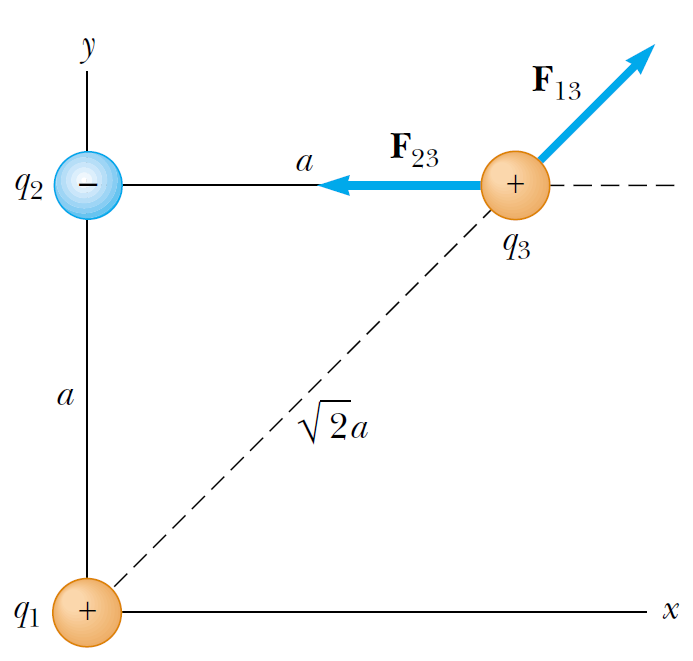
\includegraphics[scale=0.5]{Figure23-8.png}
\caption{Finding resultant force on a charge.}
\label{Resultant-force}
\end{figure}
\noindent\textbf{Question 2 \cite[Example 23.3, page 714]{Serway}:} Three charges are located in a straight line as shown in figure \ref{Zero-force}. Here $q_1=15~\mu$C and $q_2=6~\mu$C. Given that resultant force on $q_3$ is zero find the location of $q_3$.
\begin{figure}[H]
\centering
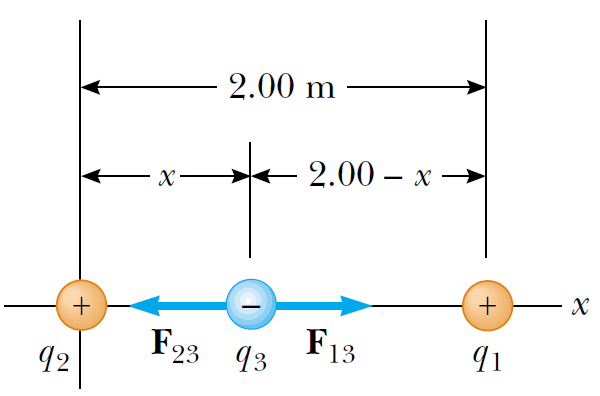
\includegraphics[scale=0.6]{Figure23-9.png}
\caption{Where is resultant force zero?}
\label{Zero-force}
\end{figure}
\noindent\textbf{Question 3 \cite[Example 23.5, page 718]{Serway}:} A charge $q1=7.0~\mu$C is located at the origin, and a second charge $q_2=-5.0~\mu$C is located on the $x$--axis, 0.30 m from the origin (Figure \ref{electric-field-two-charges}). Find the electric field at the point $P$, which has coordinates (0, 0.40) m.
\begin{figure}[H]
\centering
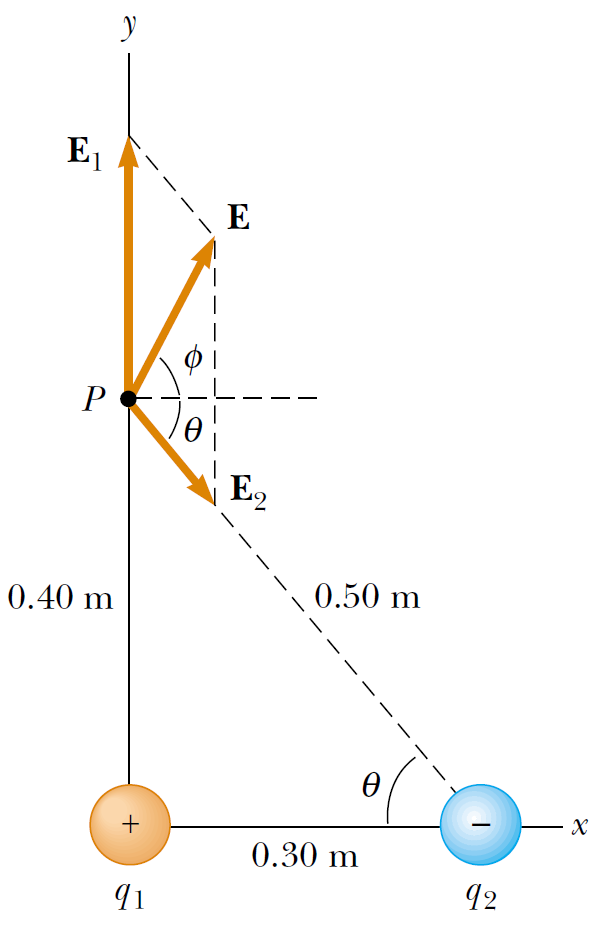
\includegraphics[scale=0.45]{Figure23-14.png}
\caption{Net electric field of two point charges.}
\label{electric-field-two-charges}
\end{figure}
\newpage
\noindent\textbf{Question 4 \cite[Example 23.6, page 719]{Serway}:} An electric dipole is defined as a positive charge $q$ and a negative charge $-q$ separated by a distance $2a$. For the dipole shown in figure \ref{electric-field-dipole}, find the electric field \textbf{E} at $P$ due to the dipole, where $P$ is a distance $y >> a$ from the origin.
\begin{figure}[H]
\centering
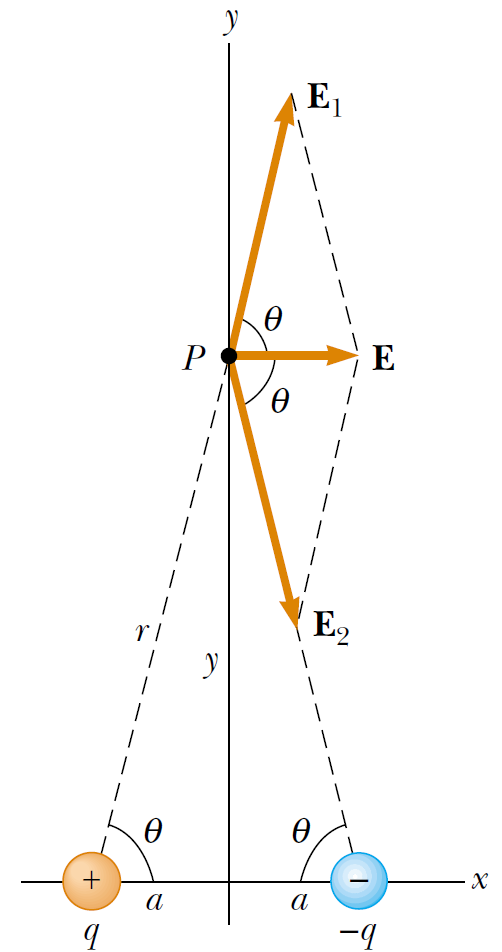
\includegraphics[scale=0.45]{Figure23-15.png}
\caption{Electric field of dipole.}
\label{electric-field-dipole}
\end{figure}
%\nocite{*}
\bibliographystyle{plain}
\bibliography{EMTRef}
\end{document}
